\documentclass[a4paper, oneside, 11pt]{scrbook}

% Get the necessary packages for the document.
% Set to english language and utf8.
\usepackage[english]{babel}
\usepackage[utf8]{inputenc}

% Some packages for symbols we need within the tutorial.
\usepackage{dingbat}
\usepackage{marvosym}

% For the sourcecode.
\usepackage{listings}

% For the links etc.
\usepackage[pdfborder={0 0 0}]{hyperref}

% For the pdf-graphics.
\usepackage{graphicx}

% The steamroller tactics to fix figures and so on.
\usepackage{float}

% This is for tables which are to long to be shown on one page.
\usepackage{longtable}

% This package is for the directory tree structures
\usepackage{dirtree}

% We need this package for some color within the document.
\usepackage{color}

% This is the package for the margin-nodes.
\usepackage[color=white, bordercolor=white]{todonotes}

\usepackage{amsfonts}
\usepackage{setspace}
\usepackage{ae,aecompl}

\usepackage[automark]{scrpage2}

\usepackage[margin=0.5cm,indention=-3em,font={sf},labelfont={bf,sf},format=hang]{caption}
% Get the new commands we defined for this document.
% The name of Kieker, just for the case that the design of this should change.
\newcommand{\Kieker}{\textsf{Kieker}}

% The current version-string.
\newcommand{\version}{1.5-trunk}

% The single parts of Kieker and some files.
\newcommand{\KiekerMonitoringPart}{\textsf{Kieker.Monitoring}}
\newcommand{\KiekerAnalysisPart}{\textsf{Kieker.Analysis}}
\newcommand{\analysisJar}{kieker-analysis-\version.jar}
\newcommand{\monitoringJar}{kieker-monitoring-\version.jar}
\newcommand{\commonJar}{kieker-common-\version.jar}
\newcommand{\toolsJar}{kieker-tools-\version.jar}
\newcommand{\commonsLoggingJar}{commons-logging-1.1.1.jar}
\newcommand{\monitoringPropertiesFile}{kieker.monitoring.properties}
\newcommand{\analysisPropertiesFile}{kieker.analysis.properties}
\newcommand{\logFourJPropertiesFile}{log4j.properties}
\newcommand{\aopFile}{aop.xml}

% The complete url where to find Kieker.
\newcommand{\KiekerURL}{\url{http://sourceforge.net/projects/kieker/files}}

% This is how we call the kieker directory.
\newcommand{\KiekerDir}{kieker-\version{}}%{$<$KIEKER-DIR$>$}

% These commands are necessary to mark classes, methods and files within the document.
\newcommand{\class}[1]{\texttt{#1}}
\newcommand{\method}[1]{\textit{#1}}
\newcommand{\dir}[1]{\texttt{#1}}
\newcommand{\file}[1]{\texttt{#1}}

% TODO command for our document
\newcommand{\TODO}[1]{\todo[inline,color=green!40]{TODO: #1}}

% These commands are for notifying the reader about something important.
\newcommand{\marginbox}[1]{\todo[noline]{#1}}
\newcommand{\notify}{\marginbox{\huge{\rightpointleft}}}
\newcommand{\warning}{\marginbox{\huge{\Stopsign}}}


% The following commands set the listings for the different (programming) languages correctly.
% For the first they use all nearly the same settings.
\newcommand{\setListing}[4]{
\lstset{
language=#1,          
numbers=#2,
basicstyle=#3,       	% the size of the fonts that are used for the code
showspaces=false,               % show spaces adding particular underscores
showstringspaces=false,         % underline spaces within strings
showtabs=false,                 % show tabs within strings adding particular underscores
%frame=shadowbox,	                % adds a frame around the code
frame=lrtb,
rulesepcolor=\color{black},
tabsize=2,	                % sets default tabsize to 2 spaces
captionpos=t,                   % sets the caption-position to bottom
breaklines=true,                % sets automatic line breaking
breakatwhitespace=false,        % sets if automatic breaks should only happen at whitespace
title=\lstname,                 % show the filename of files included with \lstinputlisting; also try caption instead of title
escapechar={#4}
}
}
\newcommand{\setJavaCodeListing}{\setListing{Java}{left}{\sffamily\scriptsize}{}}
\newcommand{\setBashListing}{\setListing{Bash}{none}{\sffamily\scriptsize}{°}}
\newcommand{\setXMLListing}{\setListing{XML}{none}{\sffamily\scriptsize}{}}


% Set the title and everything.
\title{\Kieker\ Framework\\ \Large{Continuous Monitoring and Analysis of Java Software Behavior}\\ -- Tutorial --}

% Here we go.
\begin{document}
  % We want a table of contents seperated from the rest of the text.
  \maketitle
  \tableofcontents
  \newpage

  % Insert the other parts of the document.
  \chapter{Introduction}
	\section{What is \Kieker?}

		\Kieker\ is a framework facilitating the monitoring and analysis of control flows, response times and generally the runtime behavior of Java applications. Normal ({}``plain) Java applications can be arranged with the framework as well as server based Java web applications. The framework itself has been developed with regard to providing an easy manageable, maintainable piece of software, which can be included uncomplicated into both, new and existing software projects. Kieker has been designed for a continuous operation, resulting in a very small overhead during the monitoring. Kieker can probe whole method calls as well as single statements (e.g. a = a + 1).\\ 
		Nearly every component of the framework can be extended and adjusted easily as necessary.

		% This is the component diagram of Kieker (the satellite).
		\begin{figure}[H]
			\begin{centering}
				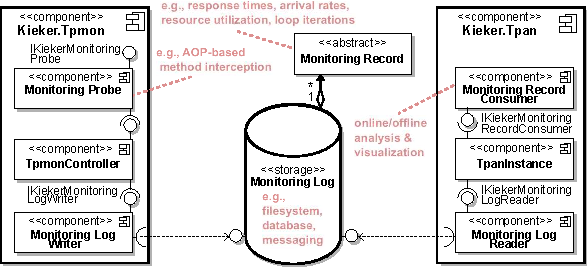
\includegraphics[width=1\textwidth]{images/kiekerComponentDiagram}
			\end{centering}
			\caption{The component diagram of \Kieker}
			\label{Figure:KiekerComponentDiagram}
		\end{figure}
		
		Figure \ref{Figure:KiekerComponentDiagram} shows that the framework consists mainly of two big parts:
		\begin{itemize}
			% Both items get notify-tags because of the important information in here.
			\item \KiekerMonitoringPart\\
			This is the part which is responsible for probing, logging and recording the program behavior. Its core is the singleton class \class{MonitoringController} \notify which receives the records and stores them into different monitoring logs, like for example into files or into databases.
			\item \KiekerAnalysisPart\\
			This part is responsible for the evalution and possible visualization of the recorded information. Its core is the class \class{AnalysisInstance} \notify which manages the lifecycle of the readers and all plugins which shoud analyze the stored informations.
		\end{itemize}
		Both parts are composed of subcomponents which can just be used or extended as well with own classes. The rough interaction between the components is described in Figure \ref{Figure:KiekerCommunicationDiagram} but will be explained furthermore in the course of this tutorial.

		% This image shows the communication diagram of the different components.
		\begin{figure}[H]
			\begin{centering}
				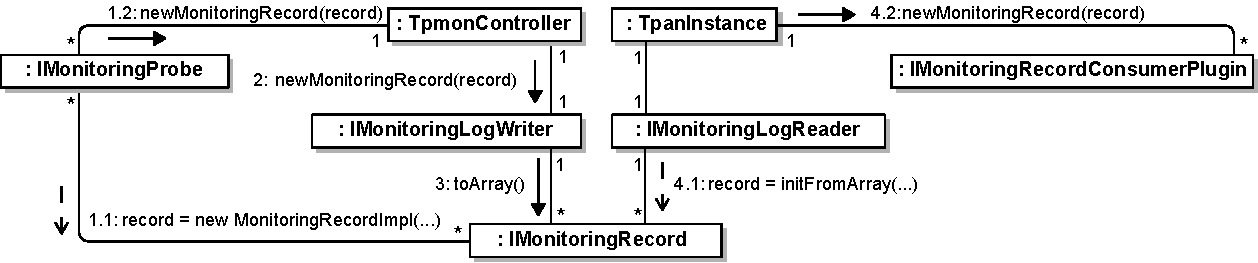
\includegraphics[width=1\textwidth]{images/kiekerCommunications-revisedReArranged-woMonitoringLog-bw}
			\end{centering}
			\caption{The communication diagram of \Kieker}
			\label{Figure:KiekerCommunicationDiagram}
		\end{figure}
		
		% Notify-tag because it is explained how Kieker works.
		\notify The monitoring probes create the monitoring records and deliver them to the monitoring controller. The monitoring controller uses the monitoring log writers to persist the given records which can later be read by a monitoring log reader who creates a monitoring record again. These records can then be used by the consumers in nearly every way.

	\section{Features}
	% This part has to be filled!
	
	\section{The purpose of this tutorial}
		% Short explanation what the tutorial will show now.
		This tutorial will take a closer look at both, the \KiekerMonitoringPart - and the \KiekerAnalysisPart-part. It will be described on the one hand how \KiekerMonitoringPart  can be used to mark parts of the own sourcecode for \Kieker\  and to let them run under surveilance, so that the recorded informations can be persisted somewhere and on the other hand \KiekerAnalysisPart will be used for processing the recorded data.\\
		Before this tutorial goes deeper into the single parts of the framework, it shows how to create and execute a simple example.
  \chapter{Example}
	% Again a short introduction.
	In this chapter a simple example will be developed by installing \Kieker\ before marking some code lines for the monitoring. After the necessary data has been collected, they will be analyzed by an own developed component.\\
	% Notify-tag because this could be interesting for the reader.
	\notify Most of the examples in this tutorial are available on the website of \Kieker.

	\section{Download and Installation}
		\Kieker\  can be downloaded from \KiekerURL. The content of the zip- respectively the tar.gz-file can be extracted to any directory, which we will call ``\KiekerDir'' within this tutorial. The installation of \Kieker\ is completed.\\
		If desired, the new created directory can be assigned to an easy remindable environment variable.


	\section{Monitoring}
		For the creation of the example is is recommended to create a new working directory (e.g. \dir{example}) of the following structure:
		\dirtree{%  
		.1 example\DTcomment{The root directory of the project}.
		.2 build\DTcomment{The directory for the compiled class files for Java}. 
		.2 lib\DTcomment{The directory for the libraries and needed jar-files}.
		.3 \monitoringJar\DTcomment{}.
		.3 \commonJar\DTcomment{}.
		.3 commons-logging-1.1.1.jar\DTcomment{}.
		.2 src\DTcomment{The directory for the sourcecode files}.
		.3 mySimpleKiekerExampleManual\DTcomment{The directory for the new package}.
		.4 CRM.java\DTcomment{One of the sourcecode files}.  
		.4 Catalog.java\DTcomment{One of the sourcecode files}.
		.4 Bookstore.java\DTcomment{One of the sourcecode files}.
		.4 BookstoreStarter.java\DTcomment{One of the sourcecode files}.
		} 
		% Linebreak because the text would be to close to the directory tree. 		

		The listed jar-files must be copied from the \Kieker\  directory:
		\begin{itemize}
			\item \dir{\KiekerDir/dist/\commonJar}
			\item \dir{\KiekerDir/dist/\monitoringJar}
			\item \dir{\KiekerDir/dist/commons-logging-1.1.1.jar}
		\end{itemize}
		The following listings show the content of the sourcecode files:
		\setJavaCodeListing       
		\lstinputlisting[caption=Bookstore.java]{source-example/manual-monitoring/src/mySimpleKiekerExampleManual/Bookstore.java}

		\begin{lstlisting}[caption=BookstoreStarter.java] 
			package mySimpleKiekerExampleManual;

			import kieker.analysis.plugin.MonitoringRecordConsumerException; 
			import kieker.analysis.reader.MonitoringLogReaderException;

			public class BookstoreStarter { 
			  public static void main(String[] args) { 
				/* Start the monitoring */ 
				Bookstore.startBookstoreRequests(); 
			  }
			} 
		\end{lstlisting}

		\lstinputlisting[caption=CRM.java]{source-example/manual-monitoring/src/mySimpleKiekerExampleManual/CRM.java}

		\lstinputlisting[caption=Catalog.java]{source-example/manual-monitoring/src/mySimpleKiekerExampleManual/Catalog.java}

		The monitoring itself is done manually. Although this is not the strength of \Kieker\ it is pretty good for a quick start. 

		% Make sure that this listing will be modified, once the sourcecode changes!!!
		% It must show the whole monitoring of the bookstorecall, from getting the first time to persisting of the record!!
		\lstinputlisting[firstline=20, lastline=29, caption=Cutting from Bookstore.java, label=listing:cuttingBookstore]{source-example/manual-monitoring/src/mySimpleKiekerExampleManual/Bookstore.java}
		
		In Listing \ref{listing:cuttingBookstore}  can be seen, how the monitoring itself is done. The time before and after a specific method call (in this case: \method{searchBook()}) is remembered. These informations are stored in the so called operation execution record. Its (partially) layout can be seen in Figure \ref{Figure:OperationExecutionRecordClassDiagram}.

		\begin{figure}[H]
			\begin{centering}
				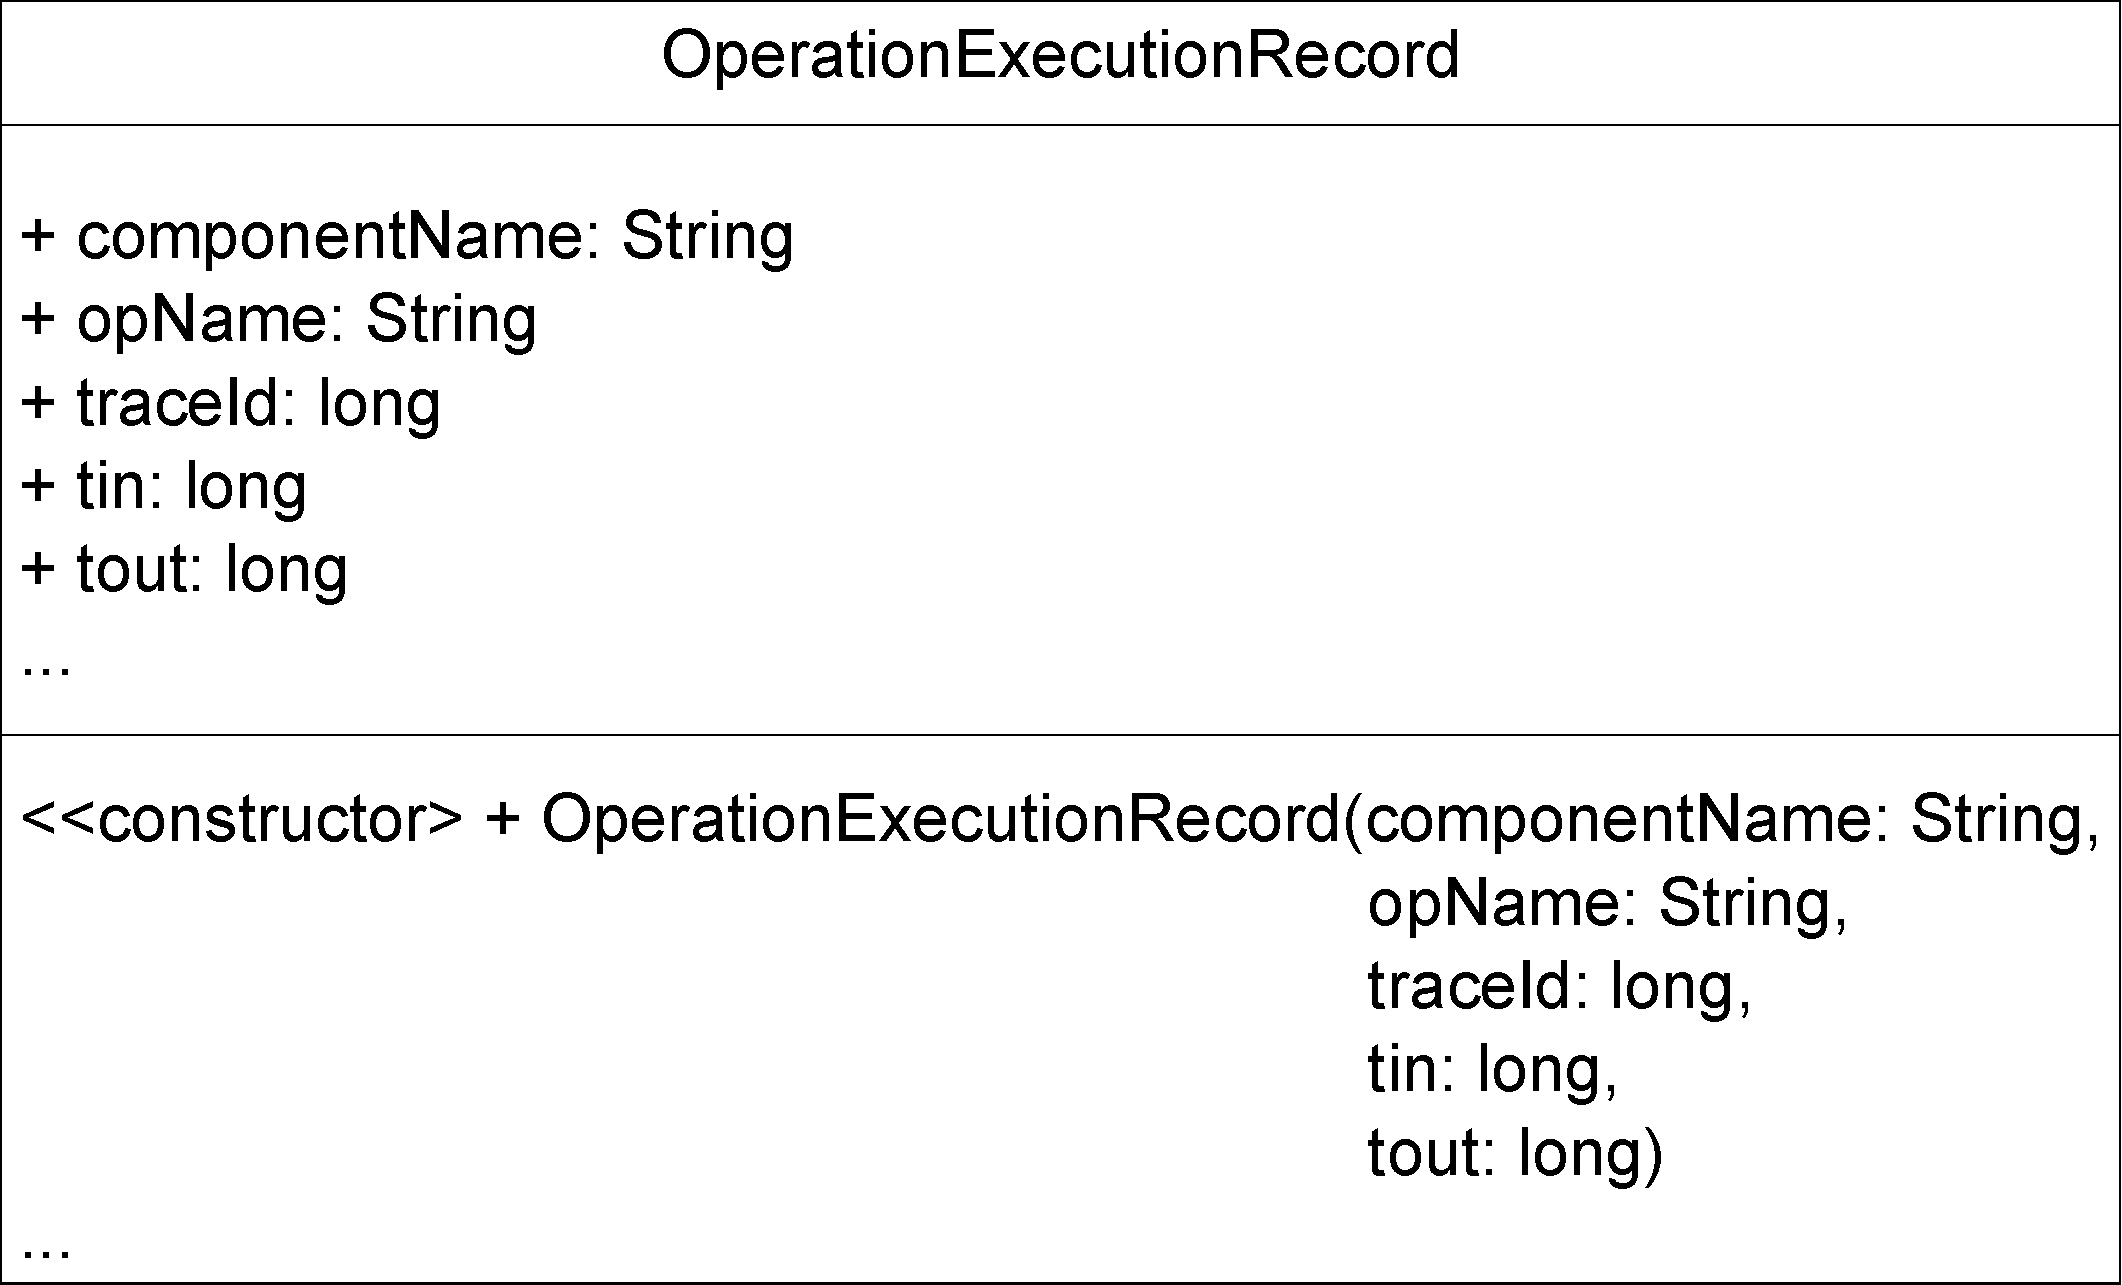
\includegraphics[width=0.4\textwidth]{images/OpExRecClassDiagram}
				\caption{The class diagram of the operation execution record}
				\label{Figure:OperationExecutionRecordClassDiagram}
			\end{centering}
		\end{figure}

		The important attributes for now are:
		\begin{itemize}
			\item componentName: The component (the class) in which the called method is.
			\item opName: The called method.
			\item traceId: The trace id of the current trace we want to record. Due to the fact, that we follow only one trace, this is zero in all recordings.
			\item tin: The time before the sourcecode which should be measured.
			\item tout: The time after the sourcecode which should be measured.
		\end{itemize}
		The sourcecode should now be compileable and executable:

		\setBashListing 		
		% Note: This is different under Windows and Linux!! 		
		% If the Kieker-Dir for the tutorial is changed, make sure that this is done here as well!! 		
		% We cannot put a latex-macro within the listing!
		\begin{lstlisting} 			
			nils@Laptop:~/example$ javac src/mySimpleKiekerExampleManual/*.java\
			-classpath\ 		
			./lib/kieker-common-1.5-trunk.jar:\
			./lib/kieker-monitoring-1.5-trunk.jar:\
			-d build

			nils@Laptop:~/example$ java\
			-Dlog4j.configuration=$<$KIEKER-DIR$>$/META-INF/log4j.properties\
			-classpath\ 	
			./build/:\
			./lib/kieker-common-1.5-trunk.jar:\
			./lib/kieker-monitoring-1.5-trunk.jar:\
			./lib/commons-logging-1.1.1.jar\
			mySimpleKiekerExampleManual.BookstoreStarter 
		\end{lstlisting}			

		% warning-tag because windows has to be handled different.
		\warning If the sourcecode should be compiled and executed under Windows, the paths have do be sepereated with semicolons instead of colons. Furthermore it is not possible to wrap the single parts of the commands with a backslash.\\
		If everything worked correctly, there should now be a new directory with the name \dir{tpmon-20100605-115948636-UTC} (just with other numbers) in the default temporary directory (under Linux this should be \dir{/tmp}; under Windows \dir{C:/temp}). In this directory, there should be a file with the extension \dir{.dat} which contains the recorded informations from the source code. A possible content of this file can be found in the appendix of this tutorial.\\
		We take now a closer look at the analysis.

	\section{Analysis}
		As mentioned in the beginning of this chapter, it is shown how a simple consumer is programmed before starting the analysis. Therefore we need some new files:

		\dirtree{%  
		.1 example.
		.2 build. 
		.2 lib.
		.3 \monitoringJar.
		.3 \color{red}\analysisJar.
		.3 \commonJar.
		.3 commons-logging-1.1.1.jar.
		.2 src.
		.3 mySimpleKiekerExampleManual.
		.4 CRM.java.  
		.4 Catalog.java.
		.4 Bookstore.java.
		.4 BookstoreStarter.java.
		.4 \color{red}Consumer.java.
		}      
		
		The new jar-file can again be found in \dir{\KiekerDir/dist}. Listing \ref{listing:Consumer} shows the content of the new created \dir{Consumer.java}. It implements the \class{IMonitoringRecordConsumerPlugin} and overrides the necessary methods so that it can later be used by the analysis component of \Kieker. In this case the component gets a maximal response time within the constructor which will later be used to check whether a recorded method call replied fast enough or not. If the method call needed more time to response that the maximal allowed response time, it will be written directly to the error stream.\\
		The methods \method{terminate} and \method{execute} don't do anything due to the fact that the consumer doesn't need any initialization. If the consumer would for example use threads then these methods would be the correct location to start and stop them.

		\setJavaCodeListing       
		\lstinputlisting[caption=Consumer.java, label=listing:Consumer]{source-example/manual-monitoring/src/mySimpleKiekerExampleManual/Consumer.java}

		We have now to extend the file \dir{BookstoreStarter.java} to analyze our recorded informations.

		\setJavaCodeListing       
		\lstinputlisting[caption=BookstoreStarter.java]{source-example/manual-monitoring/src/mySimpleKiekerExampleManual/BookstoreStarter.java}

		% notify-tag because this is a description how the analysis works.
		\notify The analysis consists of the following steps:
		\begin{itemize}
			\item Create a new instance (or more) of the class \class{AnalysisInstance}.
			\item Register the plugins which should evaluate the records.
			\item Register exactly one reader to read the stored informations.
			\item Start the analysis instance.
		\end{itemize}
		The sourccode can now be executed:

		\setBashListing 		
		% Note: This is different under Windows and Linux!! 		
		% If the Kieker-Dir for the tutorial is changed, make sure that this is done here as well!! 		
		% We cannot put a latex-macro within the listing!
		\begin{lstlisting} 			
			nils@Laptop:~/example$ javac src/mySimpleKiekerExampleManual/*.java\
			-classpath\ 		
			./lib/kieker-common-1.5-trunk.jar:\
			./lib/kieker-monitoring-1.5-trunk.jar:\
			./lib/kieker-analysis-1.5-trunk.jar:\
			-d build

			nils@Laptop:~/example$ java\
			-Dlog4j.configuration=$<$KIEKER-DIR$>$/META-INF/log4j.properties\
			-classpath\ 	
			./build/:\
			./lib/kieker-common-1.5-trunk.jar:\
			./lib/kieker-monitoring-1.5-trunk.jar:\
			./lib/kieker-analysis-1.5-trunk.jar:\
			./lib/commons-logging-1.1.1.jar\
			mySimpleKiekerExampleManual.BookstoreStarter 
		\end{lstlisting}			

		If everything worked correctly, the consumer should write something on the outputstream for every record it gets. A possible display of the run can be found in the appendix of this tutorial. 
    \chapter{\KiekerMonitoring}
    \section{Configuration}
      The monitoring part of \Kieker\ can be configured using the configuration file named ''\monitoringPropertiesFile``. This file should be copied for use to the directory ''META-INF`` of the own project and should - like the ''aop.xml`` - be copied during compiling. In order to inform \Kieker\ about this file, the following parameter should be used for the JVM:
      \begin{lstlisting}
	-Dkieker.monitoring.properties=META-INF/kieker.monitoring.properties
      \end{lstlisting}
      Most of the variables are self-explanatory and some of them will be explained in the following.

    \section{Records}
      % They are not really only part of the monitoring components, but they have to be mentioned somehow.
      As we already saw, the records are the objects which store the monitored informations somehow. They are not really part of \KiekerMonitoring\ but in order to the use in the following, we will examine them.\\
      If we want to implement an own record, it should be extend the already existing class \textit{kieker.common.record.AbstractMonitoringRecord}. The record should be able to put his complete content into an array (of Object] so that the other components of \Kieker\ are able to persist and load the data and should of course provide a method to restore the content from an array. The following listing shows a simple record implementation which has fields for the class and the method that is called.
      \setJavaCodeListing
      \lstset{caption=MyRecord.java}
      \lstinputlisting{source-example/monitoring-and-analysis-with-own-components/src/mySimpleKiekerExample/bookstoreTracing/MyRecord.java}

    \section{Probes}
      The probes are responsible for the decision which (and where) informations should be recorded. Technically we already implemented them by surrounding the method calls with the correct statements to clock, to produce the records and to deliver these records to the monitoring controller. Other specific controller could for example record only the amount of delivered bytes between methods or record only every second method call as well.\\
      We already used the annotations to make the monitoring much more comfortable and could also implement own annotations for AspectJ, but this won't be explained in this tutorial, because it would simply go beyond the scope.

    \section{Writers}
      \hypertarget{monitoringlogwriters} 
      The so called \textit{monitoring log writers} (they can be seen as well in figure \ref{image:kiekercomponentdiagram}) are the parts of \Kieker\ which are responsible for writing and serializing the recorded informations into files, databases and so on. In other words: They get an instance of \textit{AbstractKiekerMonitoringRecord} and produce an output of any nature whatsoever.\\
      Of course there are already some writers implemented, as can be seen in figure \ref{image:writers}.
      % This is the diagram with the different types of writers.
      \begin{figure}[H]
	\begin{center}
	  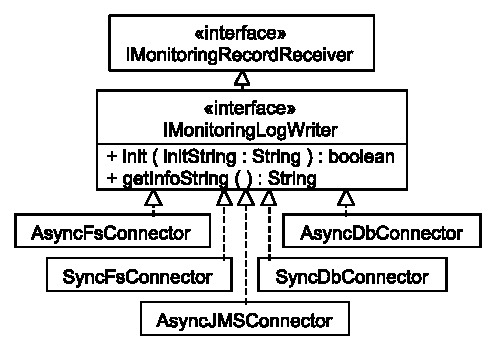
\includegraphics[width=0.5\textwidth]{kieker_writerimpls.pdf}
	  \caption{The inheritance hierarchy of the current implemented monitoring log writers}
	  \label{image:writers}
	\end{center}
      \end{figure}
      As the quick start part already showed it, every monitored record is sent to the \textit{TpmonController} which itself calls the current writer. The writer uses for example the \textit{toArray()} method of the record to get the informations stored by the record as handable array. The writer is then able to write these objects for example into a file.\\
      The implementation of an own writer class is quiet simple and can be done by implementing the interface \textit{kieker.monitoring.writer.IMonitoringLogWriter}. The following listing shows an example writer which uses a named pipe\footnote{The class \textit{MyNamedPipeManager} will be shown in the appendix of this tutorial.} to write the given records directly into the memory.
      \setJavaCodeListing
      \lstset{caption=MyWriter.java}
      \lstinputlisting{source-example/monitoring-and-analysis-with-own-components/src/mySimpleKiekerExample/bookstoreTracing/MyWriter.java}
      It is necessary to tell \KiekerMonitoring\ which writer should be used. This can be done in the already mentioned file ''\monitoringPropertiesFile``:
      \setBashListing
      \begin{lstlisting}
	monitoringDataWriter=mySimpleKiekerExample.bookstoreTracing.MyWriter
	monitoringDataWriterInitString=somePipe

	# 1.1.5 [property has been removed:] Use monitoring record type IDs

	# 1.1.6 Queue Size used to store Monitoring Records
	# Asyncronous Writers need to store Monitoring Records in an internal Queue.
	# This parameter defines the Number of Records cached. If this number is exceeded
	# Kieker will terminate with a Queue Full Exception!
	#
	asyncRecordQueueSize=8000
      \end{lstlisting}
      The first property decides which writer should be used. If we don't use any of the already implemented writers, we have to deliver the whole name of the class of the writer. The second property is an init string which can be used to initialize the writer in any way. In this case we use this parameter to tell the writer which pipe should be used. The third property is just important for asyncronous writers. It must be pointed out that the resulting init string our writer gets is of the form ''somePipe $|$ asyncRecordQueueSize=8000``. 
  \chapter{Kieker Analysis Component}
	
	% Notify-tag; this is more or less a reminding.
	\class{\KiekerAnalysisPart} is the part of \Kieker\  which is responsible for the analysis, consisting of the reader, the consumer and the analysis instance itself. To read the stored records again is task of the readers. Whatever is done with these informations is task of the consumers. They can evaluate, process or visualize the data for example. The analysis instance concerns about the lifetime and registration of the other parts. As explained in the example chapter, the analysis consists\notify  of the following steps:
	\begin{itemize}
		\item Create a new instance (or more) of the class \class{AnalysisInstance}.
		\item Register the plugins which should evaluate the records.
		\item Register exactly one reader to read the stored informations.
		\item Start the analysis instance.
	\end{itemize}

	\section{Monitoring Log Readers}

		% Warning-tag for the reader-writer-thing
		The monitoring log readers are the direct counterpart to the monitoring log writers. While a writer gets a record and writes it into files or somewhere else, the reader takes the written data and converts it into a suitable instance of \class{AbstractKiekerMonitoringRecord}. \warning This means that whenever a new writer is implemented, a corresponding reader has to be implemented as well. If one want for example to store the recorded informations in a database, one should be capable of reading these saved informations from the database again.\\
		There are already some readers implemented in \Kieker\  as can be seen in the hierarchy diagram in Figure \ref{Figure:ReaderHierarchy}.

		% This image shows the reader hierarchy.
		\begin{figure}[H]
			\begin{centering}
				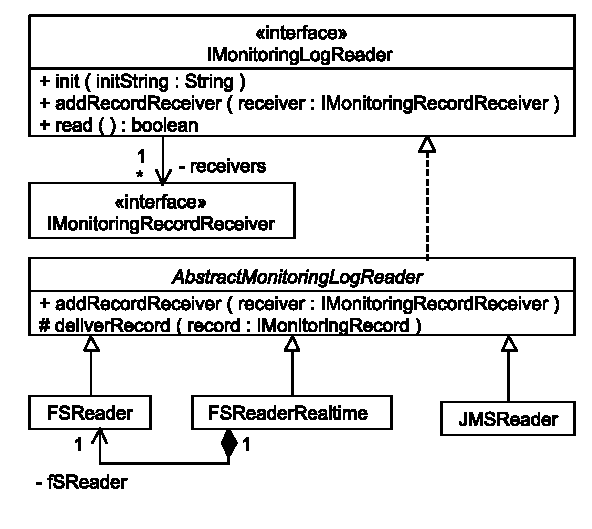
\includegraphics[width=0.5\textwidth]{images/kieker_readerimpls}
				\caption{The simple inheritance hierarchy of some currently implemented monitoring log readers}
				\label{Figure:ReaderHierarchy}
			\end{centering}
		\end{figure}

		The implementing of an own reader is nearly the same as the implementing of the writer, but to keep things simple, it is recommended to extend the already implemented AbstractKiekerMonitoringLogReader, because otherwise it would be necessary to implement the used observer pattern of the reader. By using the methods of the abstract class \class{kieker.analysis.reader.AbstractMonitoringLogReader}, the task of delivering a new record to the consumers can be delegated to the super class.\\
		The Listing \ref{listing:MyReader} shows a simple reader which reads a stored record from the pipe. If there is nothing on the pipe to be read, the reader waits 4 seconds at maximum before it terminates.

		\setJavaCodeListing
		\lstinputlisting[caption=MyReader.java, label=listing:MyReader]{source-example/monitoring-and-analysis-with-own-components/src/mySimpleKiekerExample/MyReader.java}

	\section{Record Consumer Plugins}

		The consumers are the parts of Kieker which work with the records that have been loaded by the reader. There can be (theoretically) an infinite number of consumers which produce any kind of output. A consumer can be programmed by implementing the interface \class{kieker.analysis.plugin.IMonitoringRecordConsumerPlugin} and writing the necessary methods. Following example consumer takes the given record and writes the content to the default output stream.

		\setJavaCodeListing
		\lstinputlisting[caption=MyConsumer.java]{source-example/monitoring-and-analysis-with-own-components/src/mySimpleKiekerExample/MyConsumer.java}

	\section{Analysis Instance}

		To put everything together, Listing \ref{listing:AnalysisInstance} shows how to use the above-mentioned components.

		\setJavaCodeListing
		\begin{lstlisting}[label=listing:AnalysisInstance]
AnalysisInstance ai = new AnalysisInstance();
MyReader reader = new MyReader(); 
reader.init("somePipe"); 
ai.setLogReader(reader); 	  ai.registerPlugin(new MyConsumer());
ai.run();
\end{lstlisting}
  \chapter{Trace Analysis and Monitoring}
  %%%%%%%%%%%%%%%%%%%%%%%%%%%%%%%%%%%%%%%%%
% Appendix
% 
% $Date$
% $Rev$:
% $Author$


\appendix
\renewcommand{\thesection}{\Alph{section}} \setcounter{section}{0}
\chapter*{Appendix}
\addcontentsline{toc}{chapter}{Appendix}
  \section{\KiekerMonitoringPart{} Configuration File}\label{sec:appdx:monitoringproperties}

This is the file \file{\monitoringPropertiesFile} from the binary release and 
constitutes \KiekerMonitoringPart{}'s default configuration.

\

\setXMLListing
\lstinputlisting[caption=\monitoringPropertiesFile]{../../META-INF/kieker.monitoring.properties}

\newpage


  \section{Additional Source Code Listings}
    \subsection{MyNamedPipeManager and MyPipe}
      \setJavaCodeListing
      \lstinputlisting[caption=MyNamedPipeManager.java]{\customComponentsBookstoreApplicationDir/src/bookstoreTracing/MyNamedPipeManager.java}

      \setJavaCodeListing
      \lstinputlisting[caption=MyPipe.java]{\customComponentsBookstoreApplicationDir/src/bookstoreTracing/MyPipe.java}

\newpage
  \section{Example File System Monitoring Logs}

	\subsection{Chapter \ref{chap:example}}
		The following listing shows the produced log during a run of the Bookstore Application with the manual monitoring probes.
		\setTextListing
\begin{lstlisting}[caption=Execution of the manually instrumented Bookstore application (Section~\ref{sec:example:monitoring})]
Apr 28, 2011 5:15:25 PM kieker.monitoring.core.configuration.Configuration createSingletonConfiguration
INFO: Loading properties from properties file in classpath: 'META-INF/kieker.monitoring.properties'
Apr 28, 2011 5:15:25 PM kieker.monitoring.core.configuration.Configuration loadConfigurationFromResource
WARNING: File 'META-INF/kieker.monitoring.properties' not found in classpath
Apr 28, 2011 5:15:25 PM kieker.monitoring.core.controller.MonitoringController createInstance
INFO: Current State of kieker.monitoring (1.3-20110427) Status: 'enabled'
	Name: 'KIEKER-SINGLETON'; Hostname: 'Kaapstad'; experimentID: '1'
WriterController:
	Number of Inserts: '0'
	Automatic assignment of logging timestamps: 'true'
Writer: 'kieker.monitoring.writer.filesystem.AsyncFsWriter'
	Configuration:
		kieker.monitoring.writer.filesystem.AsyncFsWriter.QueueFullBehavior='0'
		kieker.monitoring.writer.filesystem.AsyncFsWriter.QueueSize='10000'
		kieker.monitoring.writer.filesystem.AsyncFsWriter.customStoragePath=''
		kieker.monitoring.writer.filesystem.AsyncFsWriter.storeInJavaIoTmpdir='true'
	Writer Threads (1): 
		Finished: 'false'; Writing to Directory: '/tmp/kieker-20110428-151525684-UTC-Kaapstad-KIEKER-SINGLETON'
Sampling Controller: Periodic Sensor available: Current Poolsize: '0'; Scheduled Tasks: '0'
Bookstore.main: Starting request 0
Bookstore.main: Starting request 1
Apr 28, 2011 5:15:25 PM kieker.monitoring.writer.filesystem.MappingFileWriter writeMapping
INFO: Registered monitoring record type with id '1':kieker.common.record.OperationExecutionRecord
Bookstore.main: Starting request 2
Bookstore.main: Starting request 3
Bookstore.main: Starting request 4
\end{lstlisting}

		The second listing is the log during the analysis of the produced data. It can be seen that some of the calls are accepted and some others refused.
		\setTextListing
\begin{lstlisting}[caption=Execution of the example analysis (Section~\ref{sec:example:analysis})]
19.08.2010 13:19:55 kieker.analysis.AnalysisController registerPlugin
INFO: Registered plugin bookstoreApplication.Consumer@6ac2a132
19.08.2010 13:19:55 kieker.analysis.AnalysisController registerPlugin
INFO: Plugin bookstoreApplication.Consumer@6ac2a132 also registered as record consumer
19.08.2010 13:19:55 kieker.analysis.reader.filesystem.FSDirectoryReader processInputFile
INFO: < Loading C:\Temp\tpmon-20100814-103954167-UTC\tpmon-20100814-103954184-UTC-Thread-2.dat
19.08.2010 13:19:55 kieker.common.record.MonitoringRecordTypeRegistry registerRecordTypeIdMapping
INFO: Registered record type mapping 1/kieker.common.record.OperationExecutionRecord
maximal response time exceeded by 11382559 ns: bookstoreApplication.Catalog.getBook()
maximal response time exceeded by 11251720 ns: bookstoreApplication.Catalog.getBook()
maximal response time exceeded by 80320 ns: bookstoreApplication.Catalog.getBook()
maximal response time exceeded by 27400 ns: bookstoreApplication.Catalog.getBook()
maximal response time exceeded by 81760 ns: bookstoreApplication.Catalog.getBook()
maximal response time exceeded by 24240 ns: bookstoreApplication.Catalog.getBook()
maximal response time exceeded by 82480 ns: bookstoreApplication.Catalog.getBook()
response time accepted: bookstoreApplication.Catalog.getBook()
response time accepted: bookstoreApplication.Catalog.getBook()
response time accepted: bookstoreApplication.Catalog.getBook()
14.08.2010 12:41:02 kieker.analysis.reader.filesystem.FSReader$\$$FSReaderCons execute
INFO: All reader threads provided FS_READER_TERMINATION_MARKER
\end{lstlisting}
	
	\subsection{Chapter \ref{chap:aspectJ}}
	    The following listing shows the produced log during a run of the Bookstore Application, weaved with the necessary code at runtime as shown in Section \ref{sec:aspectJ:fullweaving}.
		\setTextListing
\begin{lstlisting}[caption=Execution of the Bookstore with AspectJ trace instrumentation (Section~\ref{sec:traceAnalysis:instr:AspectJ})]
Bookstore.main: Starting request 0
Apr 28, 2011 4:28:29 PM kieker.monitoring.core.configuration.Configuration createSingletonConfiguration
INFO: Loading properties from properties file in classpath: 'META-INF/kieker.monitoring.properties'
Apr 28, 2011 4:28:29 PM kieker.monitoring.core.controller.MonitoringController createInstance
INFO: Current State of kieker.monitoring (1.3-20110427) Status: 'enabled'
	Name: 'KIEKER'; Hostname: 'Kaapstad'; experimentID: '1'
WriterController:
	Number of Inserts: '0'
	Automatic assignment of logging timestamps: 'true'
Writer: 'kieker.monitoring.writer.filesystem.AsyncFsWriter'
	Configuration:
		kieker.monitoring.writer.filesystem.AsyncFsWriter.QueueFullBehavior='0'
		kieker.monitoring.writer.filesystem.AsyncFsWriter.QueueSize='10000'
		kieker.monitoring.writer.filesystem.AsyncFsWriter.customStoragePath=''
		kieker.monitoring.writer.filesystem.AsyncFsWriter.storeInJavaIoTmpdir='true'
	Writer Threads (1): 
		Finished: 'false'; Writing to Directory: '/tmp/kieker-20110428-142829399-UTC-Kaapstad-KIEKER'
Sampling Controller: Periodic Sensor available: Current Poolsize: '0'; Scheduled Tasks: '0'
Apr 28, 2011 4:28:29 PM kieker.monitoring.core.registry.ControlFlowRegistry <init>
INFO: First threadId will be 7752665283541598209
Apr 28, 2011 4:28:29 PM kieker.monitoring.writer.filesystem.MappingFileWriter writeMapping
INFO: Registered monitoring record type with id '1':kieker.common.record.OperationExecutionRecord
\end{lstlisting}



	
\newpage
  \section{Ant Scripts}
    \subsection{Chapter \ref{chap:example}}
      Following listings show the necessary \file{build.xml} and \file{build.properties} to compile and execute the manual instrumentated Bookstore Application shown in Chapter~\ref{chap:example}.
      \setXMLListing
      \lstinputlisting[caption=build.xml]{\manualInstrumentedBookstoreApplicationDir/build.xml}
      \lstinputlisting[caption=build.properties]{\manualInstrumentedBookstoreApplicationDir/build.properties}
      In order to run the analysis of the application, it is still necessary to supply the program with the path to the output directory of the monitoring. This is done via the parameter "analysis.directory", e.g.:
      \setBashListing
      \begin{lstlisting}[caption=Command to compile and run the instrumented Bookstore via ant]
#\lstshellprompt{}# ant run-analysis -Danalysis.directory /tmp/kicker-20120402-163314855-UTC-myHost-KIEKER-SINGLETON
\end{lstlisting}%-KIEKER


    \subsection{Chapter \ref{chap:componentsMonitoring} and \ref{chap:componentsAnalysis}}
      Following listings show the necessary \file{build.xml} and \file{build.properties} to compile and execute the manually instrumentated Bookstore Application with the own components shown in Chapter~\ref{chap:componentsMonitoring} and \ref{chap:componentsAnalysis}.
      \setXMLListing
      \lstinputlisting[caption=build.xml]{\customComponentsBookstoreApplicationDir/build.xml}
      \lstinputlisting[caption=build.properties]{\customComponentsBookstoreApplicationDir/build.properties}

    \subsection{Chapter \ref{chap:aspectJ}}
      Following listings show the necessary \file{build.xml} and \file{build.properties} to compile and execute the Bookstore Application instrumentated with AspectJ shown in Chapter~\ref{chap:aspectJ}.
      \setXMLListing
      \lstinputlisting[caption=build.xml]{\aspectJBookstoreApplicationDir/build.xml}
      \lstinputlisting[caption=build.properties]{\aspectJBookstoreApplicationDir/build.properties}     

\newpage
  \section{Example Graphs and Diagrams}
    \begin{figure}[H]\centering
	\subfigure[]{\label{fig:appendix:aggregatedAllocationCallTree}%
	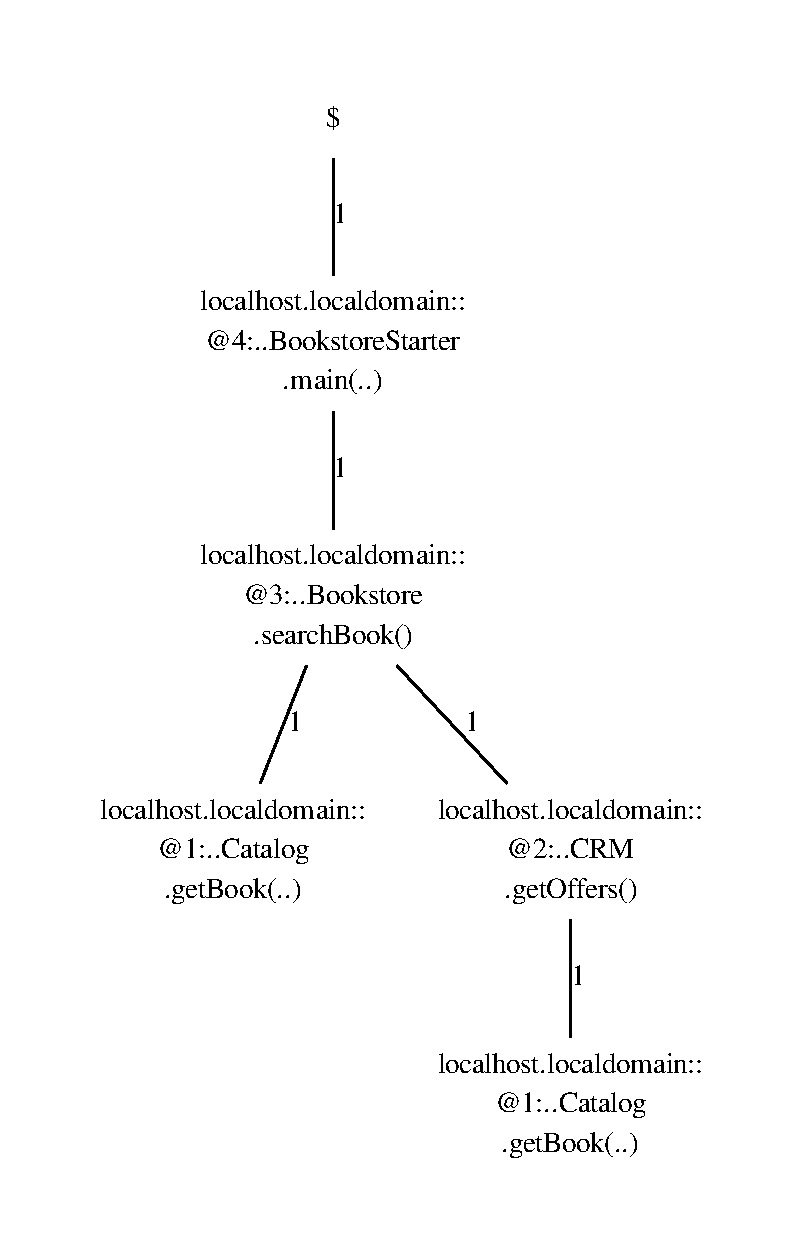
\includegraphics[width=0.33\textwidth]{images/aggregatedAllocationCallTree}%
	}%
	\subfigure[]{\label{fig:appendix:aggregatedAssemblyCallTree}%
	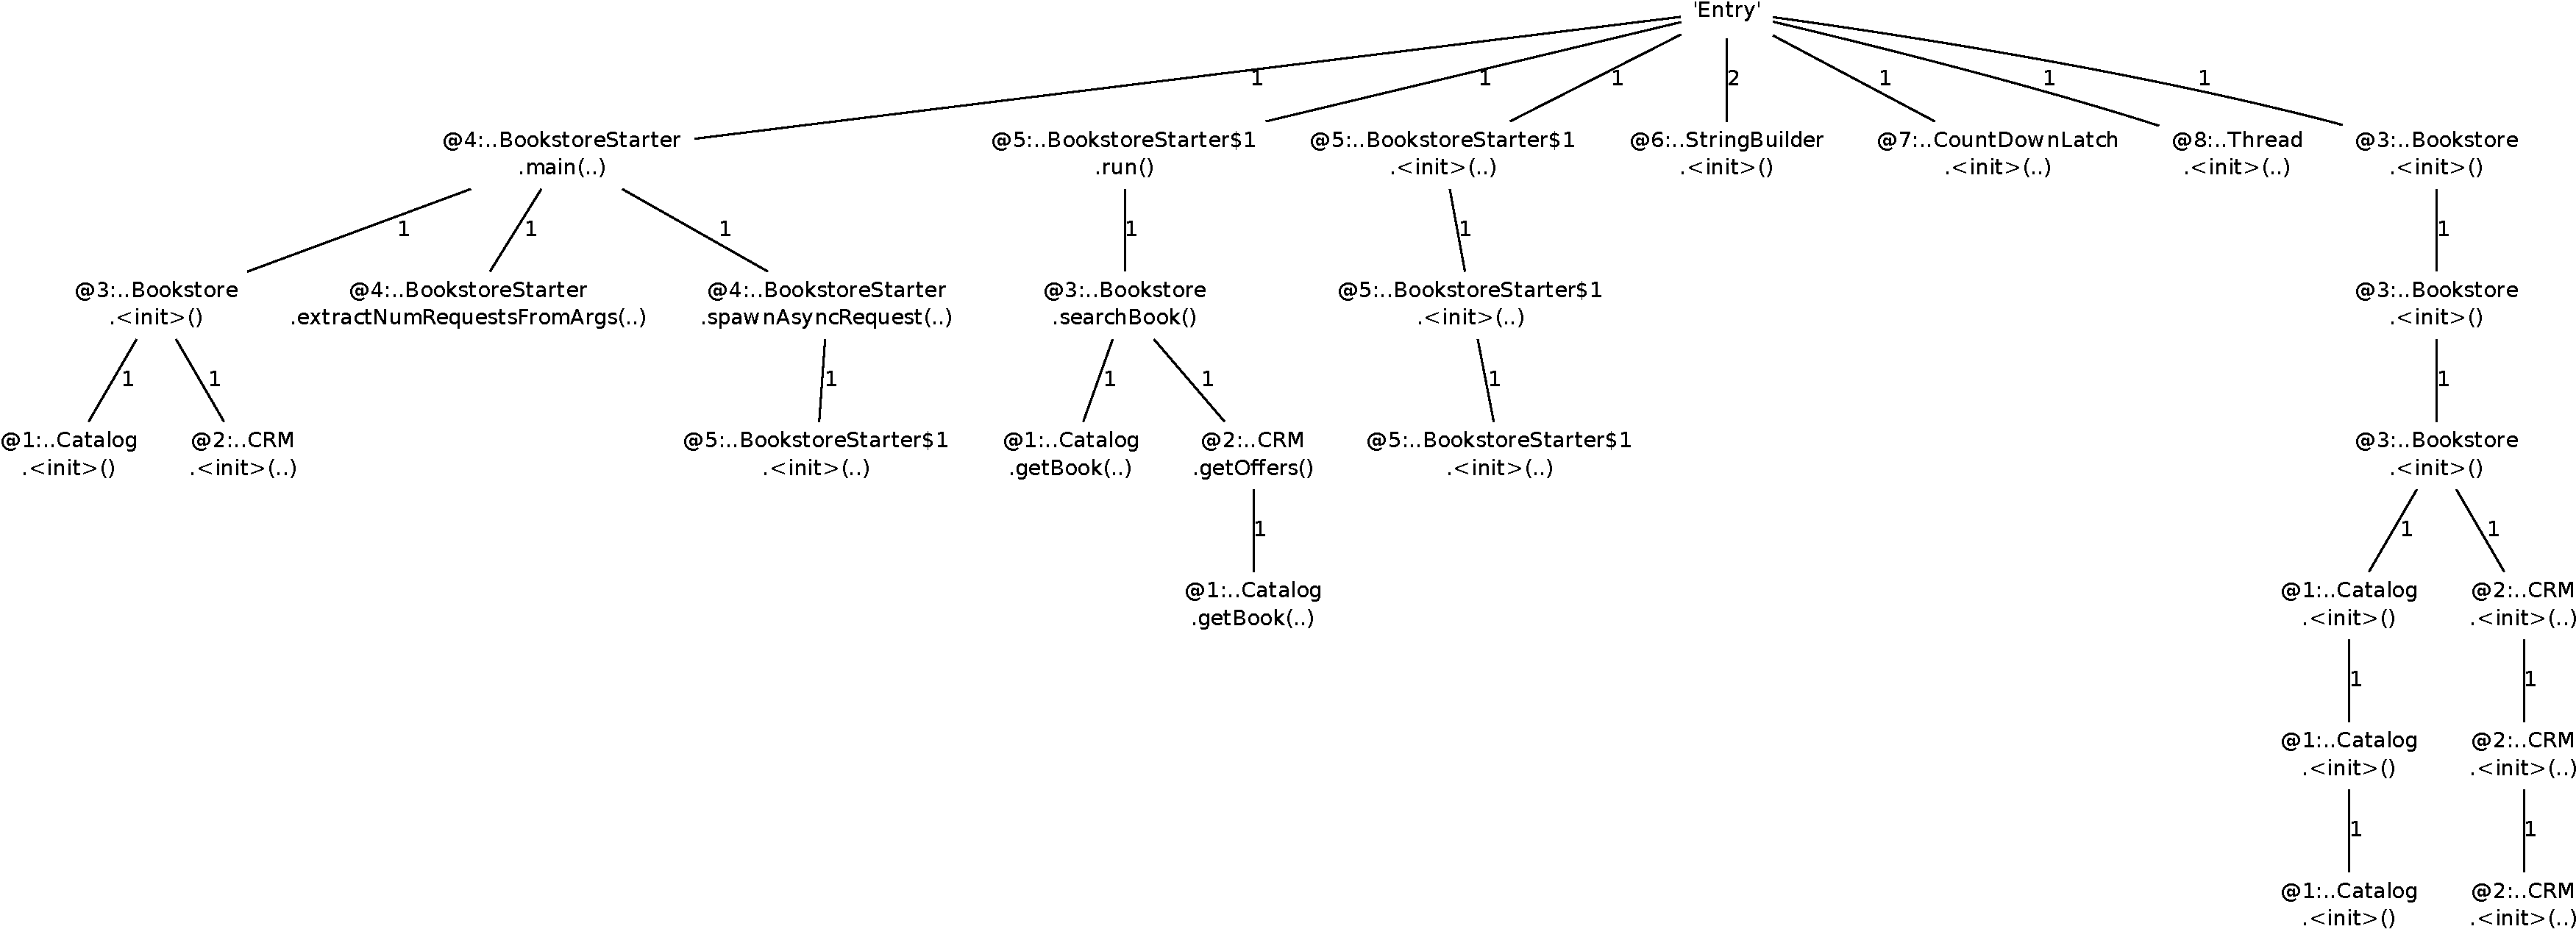
\includegraphics[width=0.33\textwidth]{images/aggregatedAssemblyCallTree}%
	}%
	\subfigure[]{\label{fig:appendix:callTree}%
	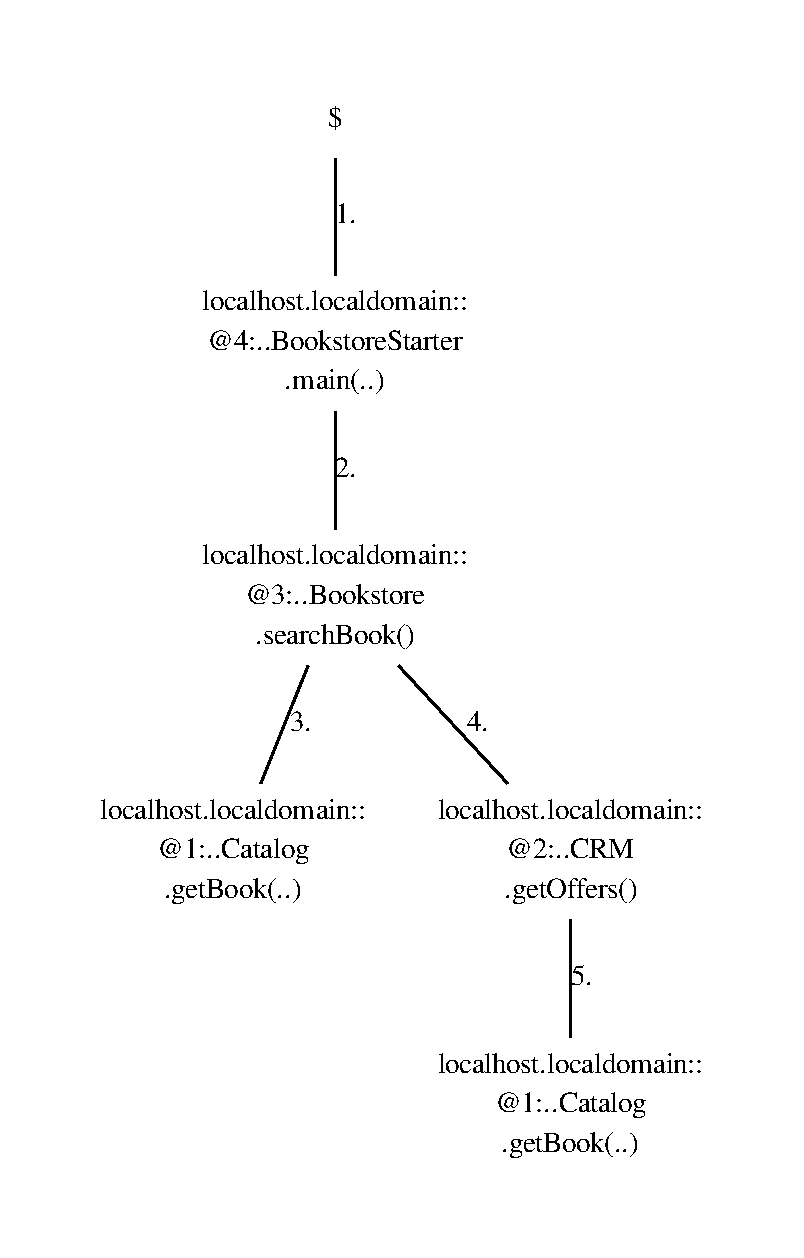
\includegraphics[width=0.33\textwidth]{images/callTree}%
	}%
	\caption{Aggregated Allocation Call Tree~\subref{fig:appendix:aggregatedAllocationCallTree}, Aggregated Assembly Call Tree~\subref{fig:appendix:aggregatedAssemblyCallTree} and Call Tree~\subref{fig:appendix:callTree}}
	\end{figure}
	
    \begin{figure}[H]\centering
	\subfigure[]{\label{fig:appendix:allocationComponentDependencyGraph}%
	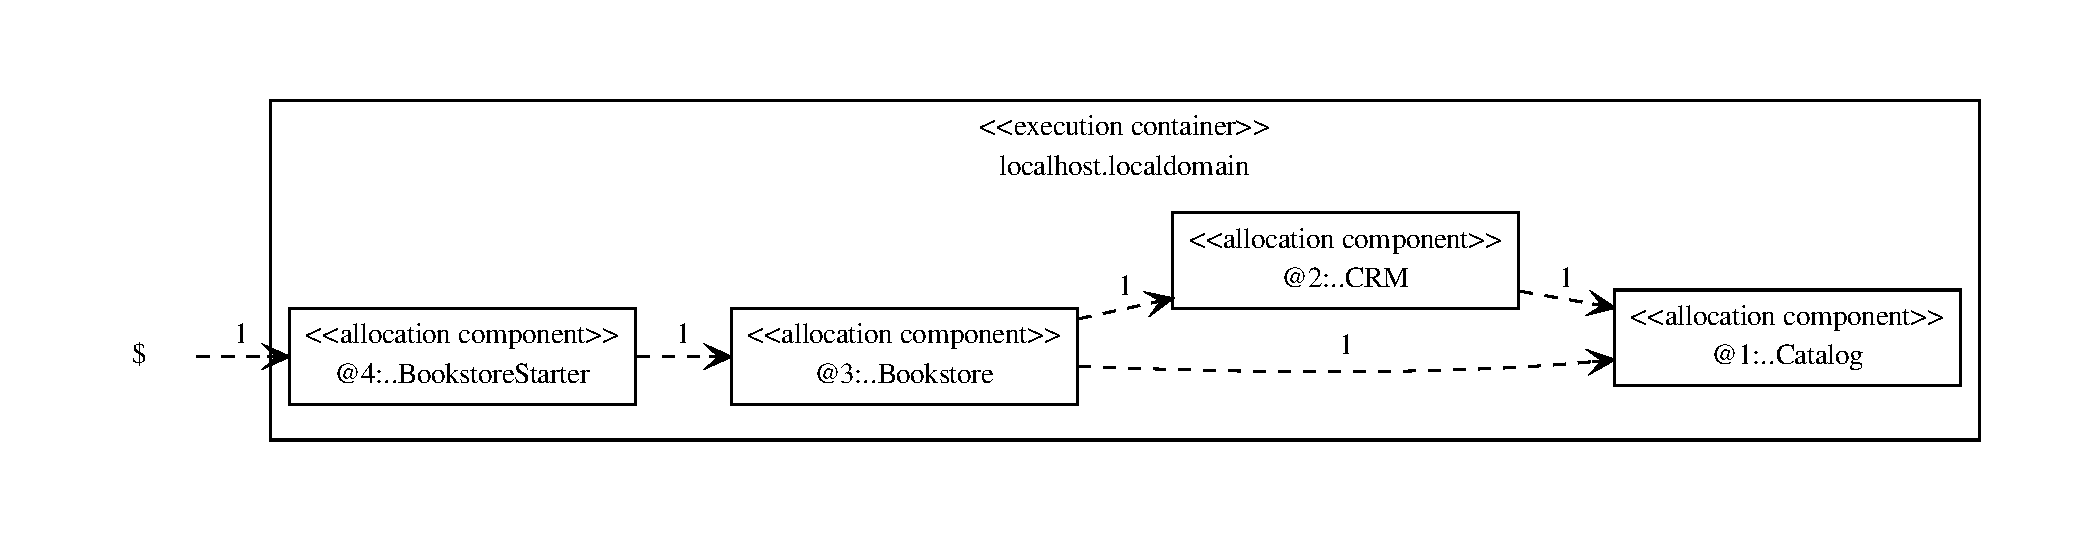
\includegraphics[width=0.8\textwidth]{images/allocationComponentDependencyGraph}
	}\\
	\subfigure[]{\label{fig:appendix:assemblyComponentDependencyGraph}%
	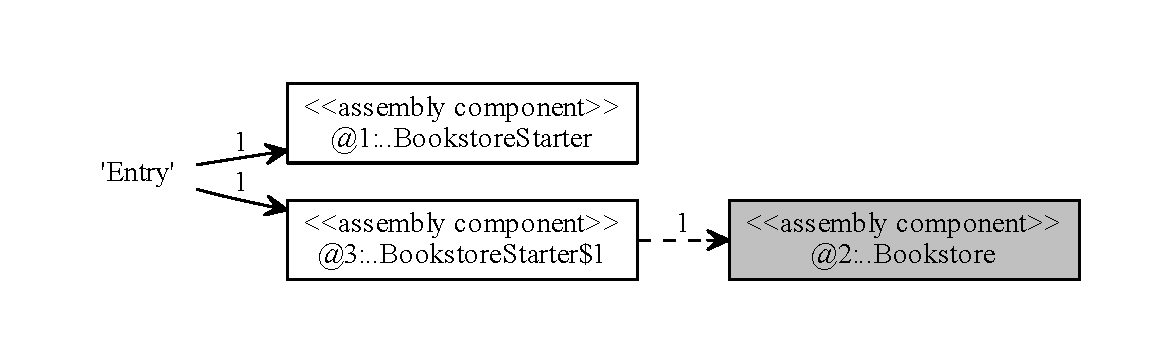
\includegraphics[width=0.8\textwidth]{images/assemblyComponentDependencyGraph}
	}%
	\caption{Allocation Component Dependency Graph~\subref{fig:appendix:allocationComponentDependencyGraph} and Assembly Component Dependency Graph~\subref{fig:appendix:assemblyComponentDependencyGraph}}
	\end{figure}
	
	\begin{figure}[H]\centering
	\subfigure[]{\label{fig:appendix:allocationOperationDependencyGraph}%
	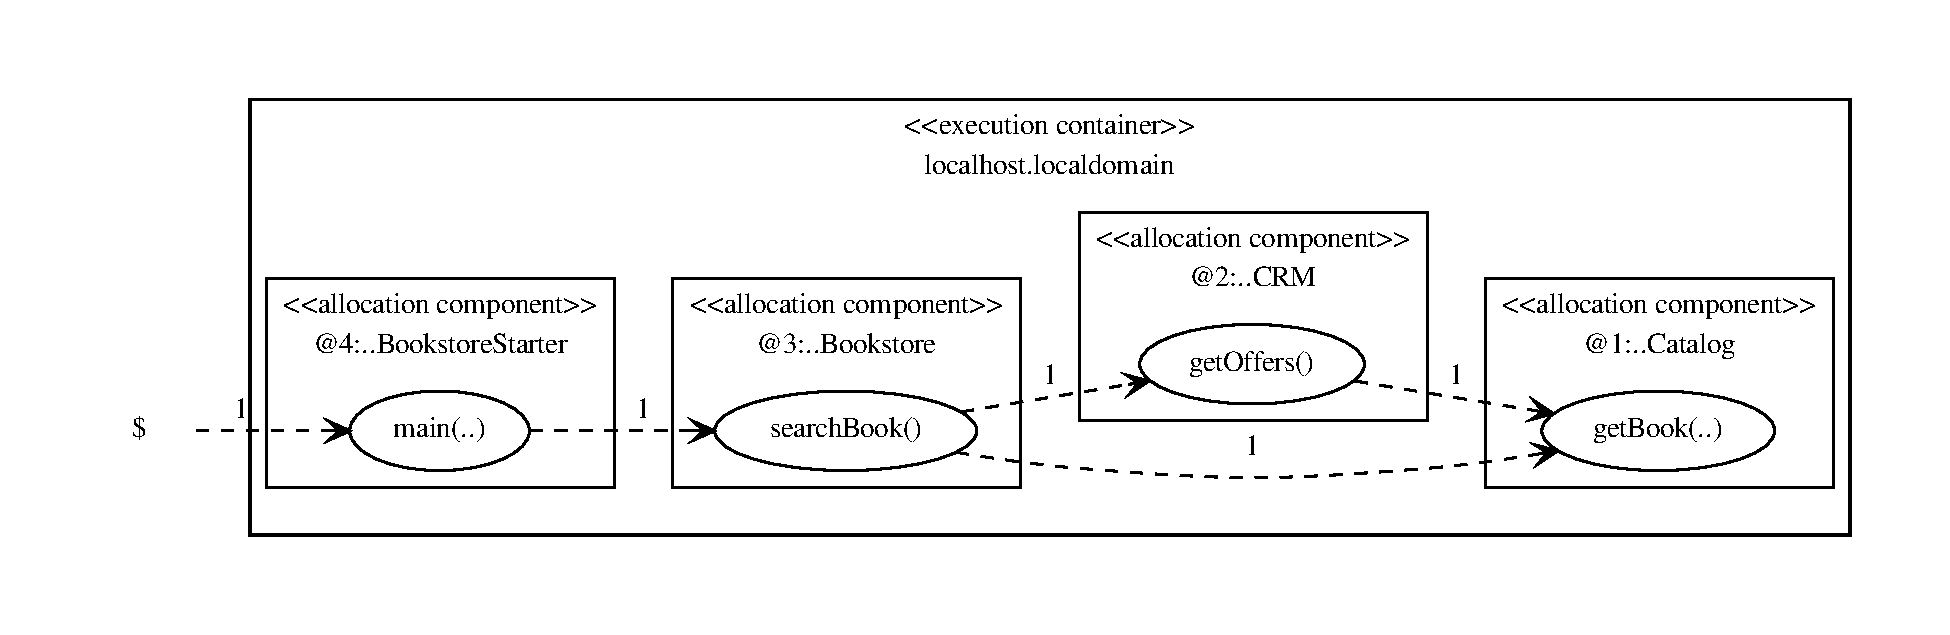
\includegraphics[width=0.8\textwidth]{images/allocationOperationDependencyGraph}
	}\\
	\subfigure[]{\label{fig:appendix:assemblyOperationDependencyGraph}%
	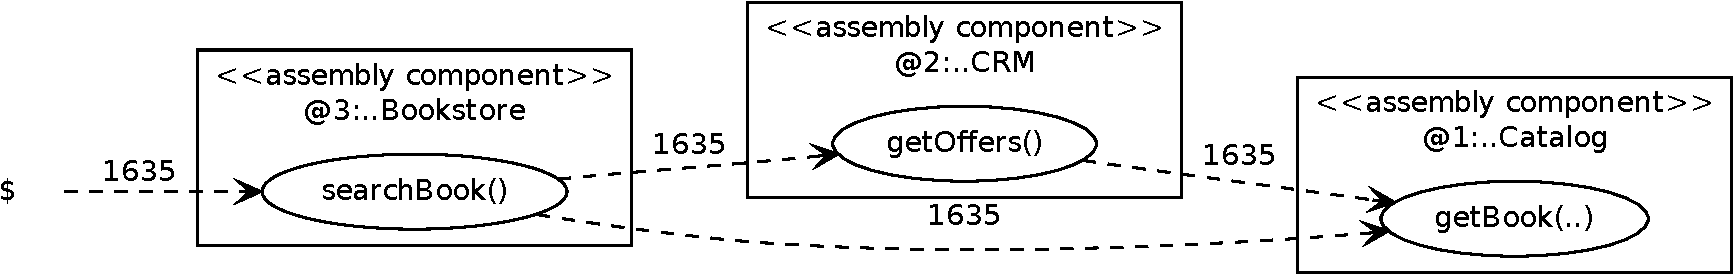
\includegraphics[width=0.8\textwidth]{images/assemblyOperationDependencyGraph}
	}%
	\caption{Allocation Operation Dependency Graph~\subref{fig:appendix:allocationOperationDependencyGraph} and Allocation Operation Dependency Graph~\subref{fig:appendix:assemblyOperationDependencyGraph}}
	\end{figure}
	
	\begin{figure}[H]\centering
	\subfigure[]{\label{fig:appendix:allocationSequenceDiagram}
	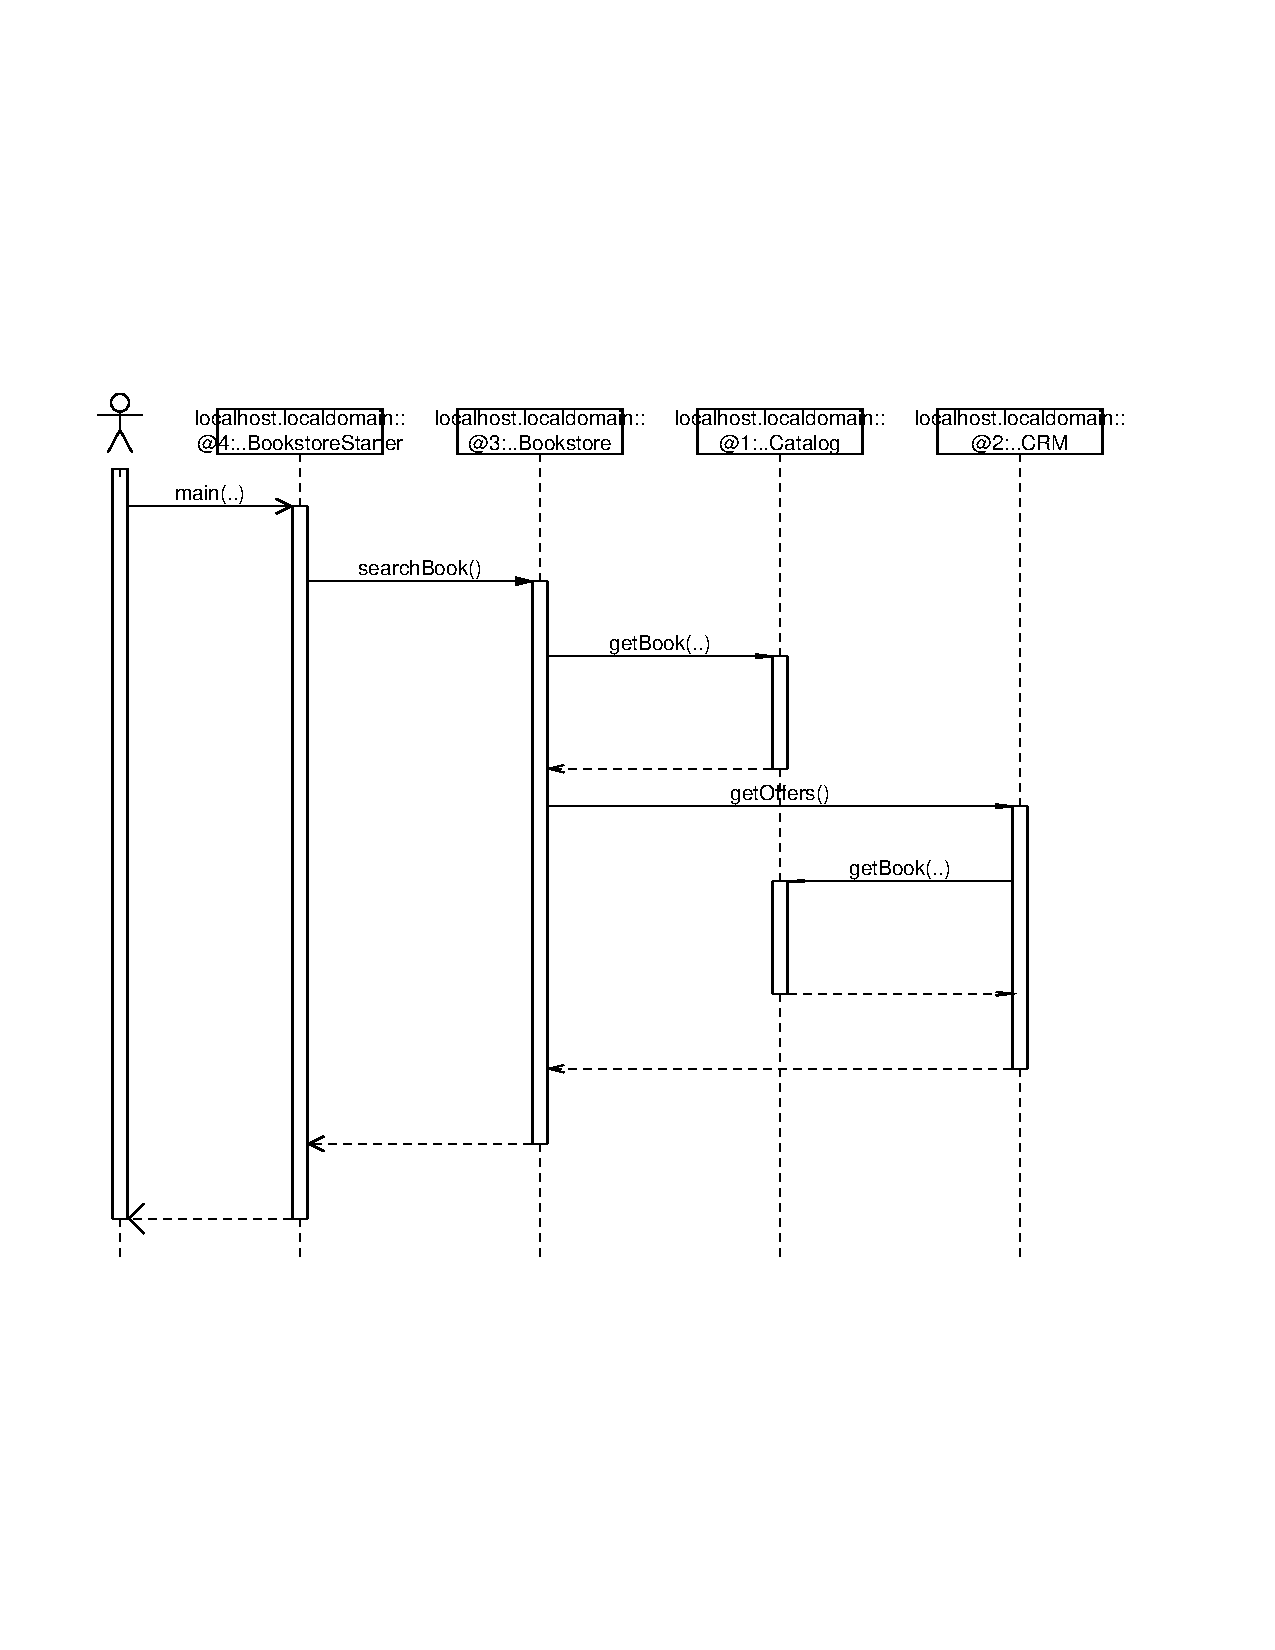
\includegraphics[width=0.4\textwidth]{images/allocationSequenceDiagram}
	}
	\subfigure[]{\label{fig:appendix:assemblySequenceDiagram}
	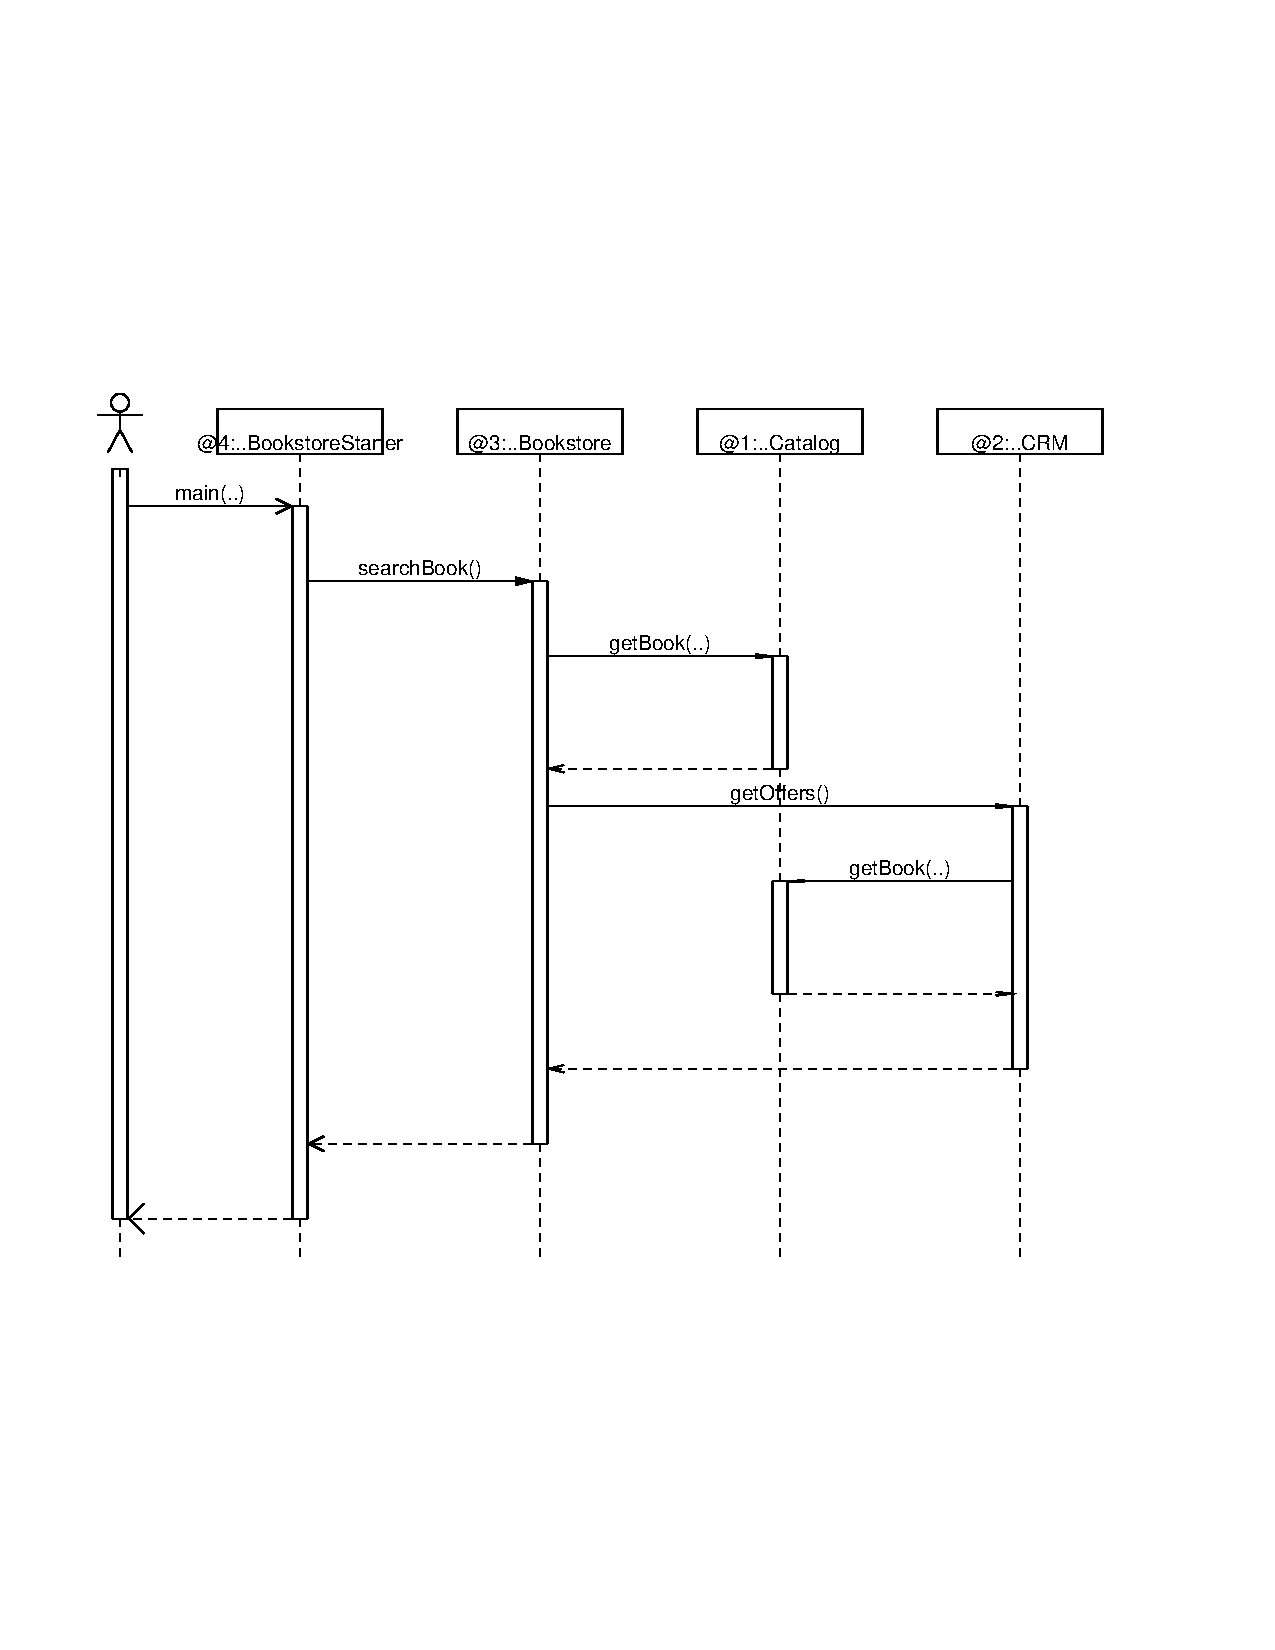
\includegraphics[width=0.4\textwidth]{images/assemblySequenceDiagram}
	}
	\caption{Allocation Sequence Diagram~\subref{fig:appendix:allocationSequenceDiagram} and Assembly Sequence Diagram~\subref{fig:appendix:assemblySequenceDiagram}}
	\end{figure}
	
	\begin{figure}[H]
		\centering
		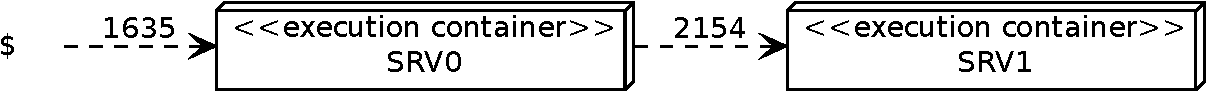
\includegraphics[width=0.5\textwidth]{images/containerDependencyGraph}
		\caption{Container Dependency Graph}
	\end{figure}
  
  
\newpage
  \section{Libraries}
    The following table shows all libraries which are used by \Kieker\ and explains them briefly.
    \begin{center}
\begin{longtable}{|p{0.4\textwidth}|p{0.5\textwidth}|}
\hline 
Filename & Description\\
\hline
\hline 
commons-cli-1.2.jar & n/a\\
\hline 
maven & n/a\\
\hline 
mysql-connector-java-5.1.5-bin.jar & The library to connect to an existing MySQL database.\\
\hline 
spring-web.jar & n/a\\
\hline 
Scenario.jar & n/a\\
\hline 
sequence.pic & n/a\\
\hline 
openjms-0.7.7-beta-1.tar.gz & n/a\\
\hline 
aspectjrt-1.6.6.jar & n/a\\
\hline 
commons-logging-1.1.1.jar & n/a\\
\hline 
aspectjtools-1.6.6.jar & n/a\\
\hline 
jms-1.1.jar & n/a\\
\hline 
concurrent-1.3.4.jar & n/a\\
\hline 
servlet.jar & n/a\\
\hline 
pmd & n/a\\
\hline 
spring.jar & n/a\\
\hline 
openjms-common-0.7.7-beta-1.jar & n/a\\
\hline 
servlet-api.jar & n/a\\
\hline 
commons-pool-1.2.jar & n/a\\
\hline 
derby.jar & This library contains the necessary drivers for the Apache Derby database.\\
\hline 
commons-io-1.2.jar & n/a\\
\hline 
cxf-rt-core-2.2.6.jar & n/a\\
\hline 
jmc.jar & n/a\\
\hline 
log4j-1.2.15.jar & n/a\\
\hline 
openjms-net-0.7.7-beta-1.jar & n/a\\
\hline 
aspectjweaver-1.6.6.jar & n/a\\
\hline 
cxf-api-2.2.6.jar & n/a\\
\hline 
rabbitmq-client.jar & n/a\\
\hline 
openjms-0.7.7-beta-1.jar & n/a\\
\hline 
spice-jndikit-1.2.jar & n/a\\
\hline 
cxf-rt-bindings-soap-2.2.6.jar & n/a\\
\hline 
cxf-common-utilities-2.2.6.jar & n/a\\
\hline 
jndi-1.2.1.jar & n/a\\
\hline 
\end{longtable}
\label{tabular:libraries}
\end{center}


% \chapter{Troubleshooting}


\end{document}
 
